% =====================================================================
%  Seance 1 -- C. Le croisement AIOps (frames 25--33)
% =====================================================================
\section{Le croisement : pourquoi le ML pour les opérations}

\begin{frame}{AIOps : le problème que le seuil fixe ne résout pas}
\footnotesize%
\begin{columns}[t]
\begin{column}{0.52\textwidth}
\begin{block}{La supervision « classique » en une ligne}
\py{if cpu > 90: alerte()} \quad --- un seuil \textbf{constant}, écrit à la main.
\end{block}
\begin{ebox}[Testé sur les vraies données NOSYS]
Sur les 69 120 fenêtres du mois, le seuil 90 \% détecte
\textbf{136 fenêtres} --- et ce sont \textbf{exactement} les 136 fenêtres
d'incident (0 faux positif, 0 raté). Verdict honnête :
\textbf{ce mois-ci, le seuil fixe fonctionne}.
\end{ebox}
\begin{wbox}[Pourquoi on n'en reste pas là]
\begin{enumerate}
\item \textbf{Chance structurelle} : le trafic normal plafonne à 55 \% de CPU ---
le seuil à 90 \% ne peut pas être dépassé hors incident. Un mois de trafic
différent (campagne, sauvegarde massive) créerait des \textbf{faux positifs}.
\item \textbf{Aveugle aux dégradations lentes} : une fuite mémoire qui monte
de +0,5 \%/jour ne franchit jamais le seuil avant la panne.
\item \textbf{Ignorant du contexte} : le même niveau n'a pas le même sens à 3 h
et à 14 h (saisonnalité jour/nuit mesurée : 10,0 \% vs 30,2 \%).
\end{enumerate}
\end{wbox}
\end{column}
\begin{column}{0.44\textwidth}
\begin{center}
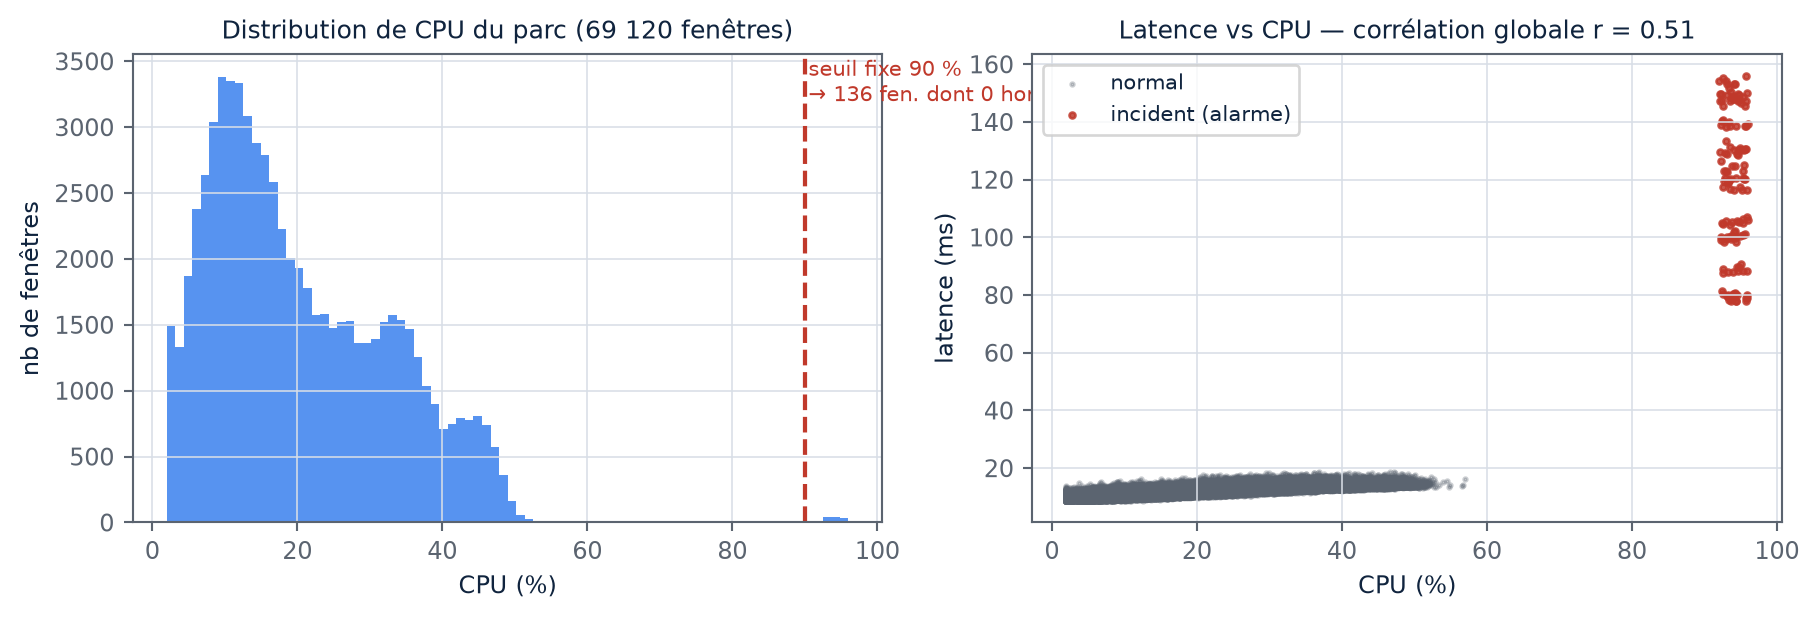
\includegraphics[width=\textwidth]{f05_seuil_vs_scatter.png}
\end{center}
\vspace{1mm}
\begin{kbox}[La bonne question]
Pas « au-dessus de quel seuil ? » mais
« \textbf{ce comportement est-il improbable} pour ce serveur, à cette heure,
dans cet état de charge ? ». C'est la définition d'un modèle.
\end{kbox}
\end{column}
\end{columns}
\end{frame}

\begin{frame}{La saisonnalité : le « normal » dépend de l'heure}
\begin{center}
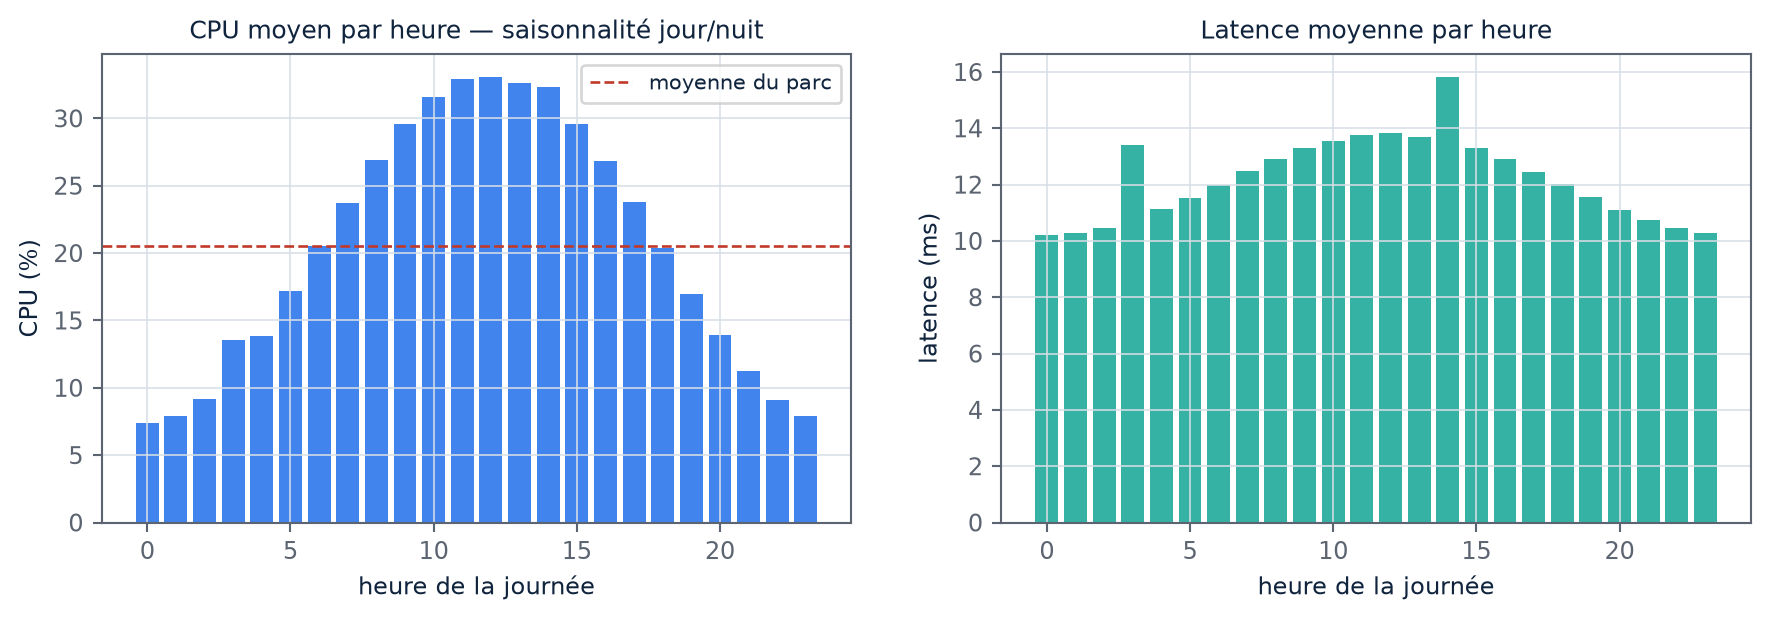
\includegraphics[width=0.92\textwidth]{f02_saisonnalite.png}
\end{center}
\begin{columns}[t]
\begin{column}{0.48\textwidth}
\begin{ebox}[Chiffres mesurés]
CPU moyen du parc : \textbf{30,2 \%} aux heures ouvrées (9 h--17 h),
\textbf{10,0 \%} la nuit (23 h--4 h) --- soit un \textbf{facteur 3}.
La latence suit le même profil.
\end{ebox}
\end{column}
\begin{column}{0.48\textwidth}
\begin{kbox}[Conséquence méthodologique]
Tout modèle sérieux encode le contexte temporel :
\textbf{heure, jour de semaine} (encodage cyclique, séance 2),
sinon il confond « 30 \% à 14 h » (normal) et « 30 \% à 3 h » (anomalie).
\end{kbox}
\end{column}
\end{columns}
\end{frame}

\begin{frame}{Zoom sur un incident : ce que le futur modèle verra}
\footnotesize%
\begin{center}
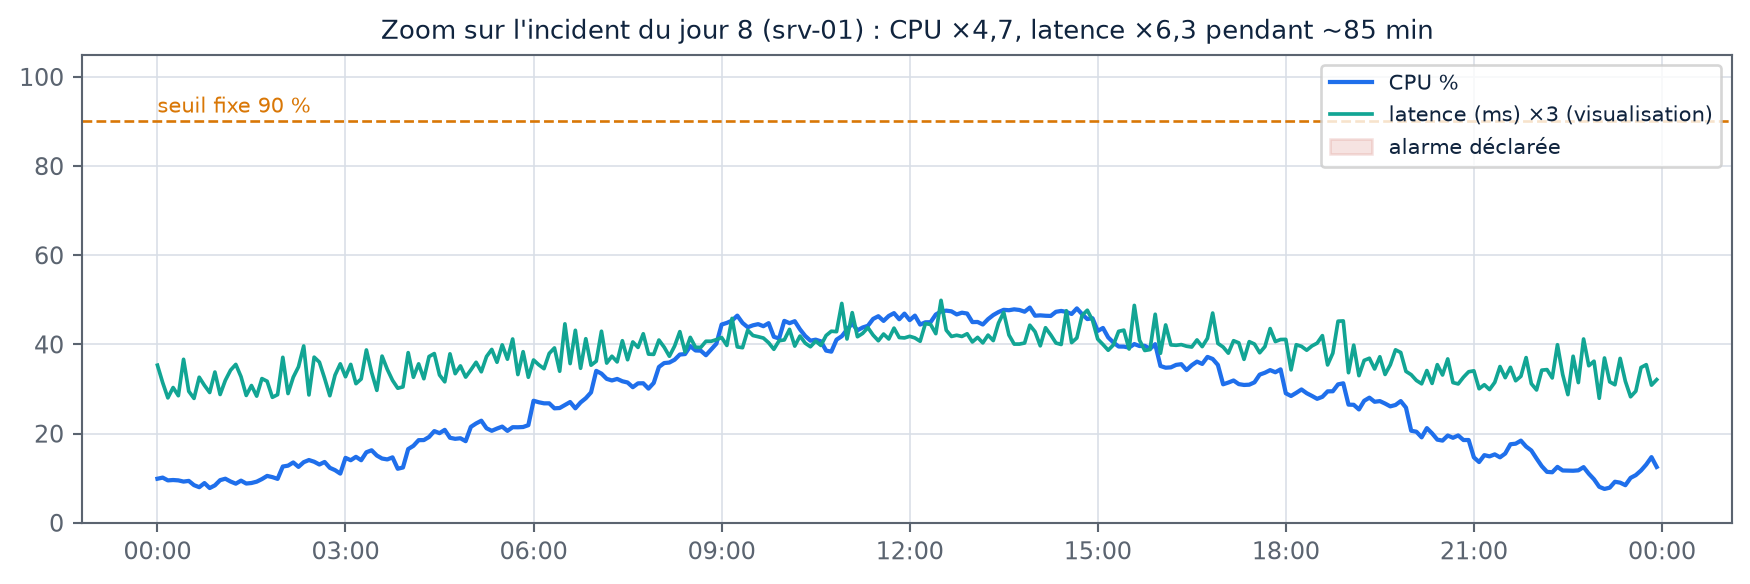
\includegraphics[width=0.94\textwidth]{f07_zoom_incident.png}
\end{center}
\begin{columns}[t]
\begin{column}{0.55\textwidth}
\begin{ebox}[Le jour 8 de srv-01 (incident réel du dossier)]
\begin{itemize}
\item Début \textbf{14 h 00}, durée \textbf{35 min} (7 fenêtres de 5 min).
\item CPU : de $\approx$ 30 \% à \textbf{95,7 \%} ($\times$ 3,2).
\item Latence : jusqu'à \textbf{156,1 ms} ($\times$ 12,8 vs p99 normal).
\item Perte de paquets multipliée par $\approx$ 5 pendant l'incident.
\end{itemize}
\end{ebox}
\end{column}
\begin{column}{0.41\textwidth}
\begin{kbox}[La question des séances 3--4]
Sur la \textbf{fenêtre de 14 h 00}, avant le pic : quels signaux précèdent
la montée ? Une \textbf{dérive} de RAM ? Une latence qui « pousse » ?
C'est exactement l'apprentissage supervisé de la cible
« incident dans les 30 min ».
\end{kbox}
\end{column}
\end{columns}
\end{frame}

\begin{frame}{La boucle AIOps complète}
\begin{center}
\begin{tikzpicture}[node distance=3.5mm and 7mm,
  box/.style={rectangle,rounded corners=2mm,draw,align=center,font=\scriptsize,
    minimum height=9mm,text width=2.9cm}]
\node[box,draw=byBlue,fill=byBlue!8]   (don) {\textbf{1. Collecter}\\métriques, logs, events\\(séances 1--2)};
\node[box,draw=byCyan,fill=byCyan!8,right=of don]  (mod) {\textbf{2. Modéliser}\\anomalies, classification,\\prévision (séances 3--4)};
\node[box,draw=byOrange,fill=byOrange!8,right=of mod] (ale) {\textbf{3. Alerter}\\seuil sur le score,\\budget d'alertes/jour};
\node[box,draw=byGreen,fill=byGreen!8,below=of ale] (act) {\textbf{4. Agir}\\runbook, autoscaling,\\équipe NOC};
\node[box,draw=byPurple,fill=byPurple!8,left=of act] (mes) {\textbf{5. Mesurer}\\l'alerte était-elle\\juste ? ré-entraîner};
\draw[-{Stealth},thick] (don) -- (mod);
\draw[-{Stealth},thick] (mod) -- (ale);
\draw[-{Stealth},thick] (ale) -- (act);
\draw[-{Stealth},thick] (act) -- (mes);
\draw[-{Stealth},thick] (mes) -- (don);
\end{tikzpicture}
\end{center}
\vspace{1mm}
\begin{itemize}
\item La boucle se \textbf{ferme} : chaque alerte jugée (juste/fausse) redevient
une \textbf{donnée d'entraînement} --- c'est ce qui distingue un AIOps vivant
d'un modèle figé.
\item Chaque séance de cette UE remplit une case de cette boucle ;
la séance 6 l'\textbf{industrialise} (API, retraining).
\end{itemize}
\end{frame}

\begin{frame}{Les quatre usages du ML en infrastructure --- la carte de l'UE}
\begin{center}
\small
\begin{tabular}{@{}p{3.4cm}p{5.2cm}p{2.2cm}p{3.4cm}@{}}
\toprule
\textbf{Usage} & \textbf{Question} & \textbf{Famille ML} & \textbf{Séance}\\
\midrule
Détection d'anomalies & Cette fenêtre est-elle improbable ? & Non supervisé & 3\\
\addlinespace[1pt]
Classification d'incident & Une panne dans les 30 min ? & Supervisé (classe rare) & 3--4\\
\addlinespace[1pt]
Prévision de charge & Quel trafic demain à 14 h ? & Séries temporelles & 4\\
\addlinespace[1pt]
Sécurité & Ces échecs d'auth forment-ils une attaque ? & Les deux & 5\\
\addlinespace[1pt]
Industrialisation & Le modèle survit-il en production ? & MLOps & 6\\
\bottomrule
\end{tabular}
\end{center}
\vspace{1mm}
\begin{kbox}[Ce que cette carte vous promet]
À la fin de l'UE, vous saurez \textbf{implémenter et déployer} chacun des
4 premiers usages sur des données réelles, et \textbf{expliquer} le cinquième.
\end{kbox}
\end{frame}

\begin{frame}{Quiz 3 --- AIOps (4 min)}
\footnotesize%
\begin{qbox}[3 questions]
\begin{enumerate}
\item Sur le mois NOSYS, le seuil fixe 90 \% a détecté 136/136 fenêtres d'incident.
Pourquoi ne pas s'arrêter là ?\\
(a) c'est de la chance structurelle : le trafic normal plafonne à 55 \% ;
dérives lentes et changement de trafic le contournent\\
(b) il faut un GPU\\ (c) le seuil était trop bas
\item La corrélation latence--CPU vaut 0,51 sur tout le mois mais
\textbf{0,80 hors incidents}. Interprétation la plus plausible ?\\
(a) la corrélation est instable \quad (b) les incidents créent des points
extrêmes qui écrasent la relation normale \quad (c) il y a une erreur de calcul
\item La boucle AIOps se distingue d'un simple modèle par\ldots\\
(a) son coût \quad (b) la mesure en boucle : chaque alerte jugée redevient
une donnée d'entraînement \quad (c) l'usage d'algorithmes plus récents
\end{enumerate}
\end{qbox}
\vspace{1mm}
\begin{solbox}[Réponses]
\textbf{1 : a} \quad \textbf{2 : b} --- c'est un effet classique des outliers ;
on le reverra (robustesse, séance 2). \quad \textbf{3 : b}
\end{solbox}
\end{frame}
